\documentclass[border=10pt]{standalone}
\usepackage[svgnames]{xcolor}
\usepackage{amsmath}
\usepackage{pgfplots}
\pgfplotsset{compat=newest}
\usepackage[sfdefault]{FiraSans}
\usepackage{FiraMono}
\renewcommand*\familydefault{\sfdefault}
\begin{document}
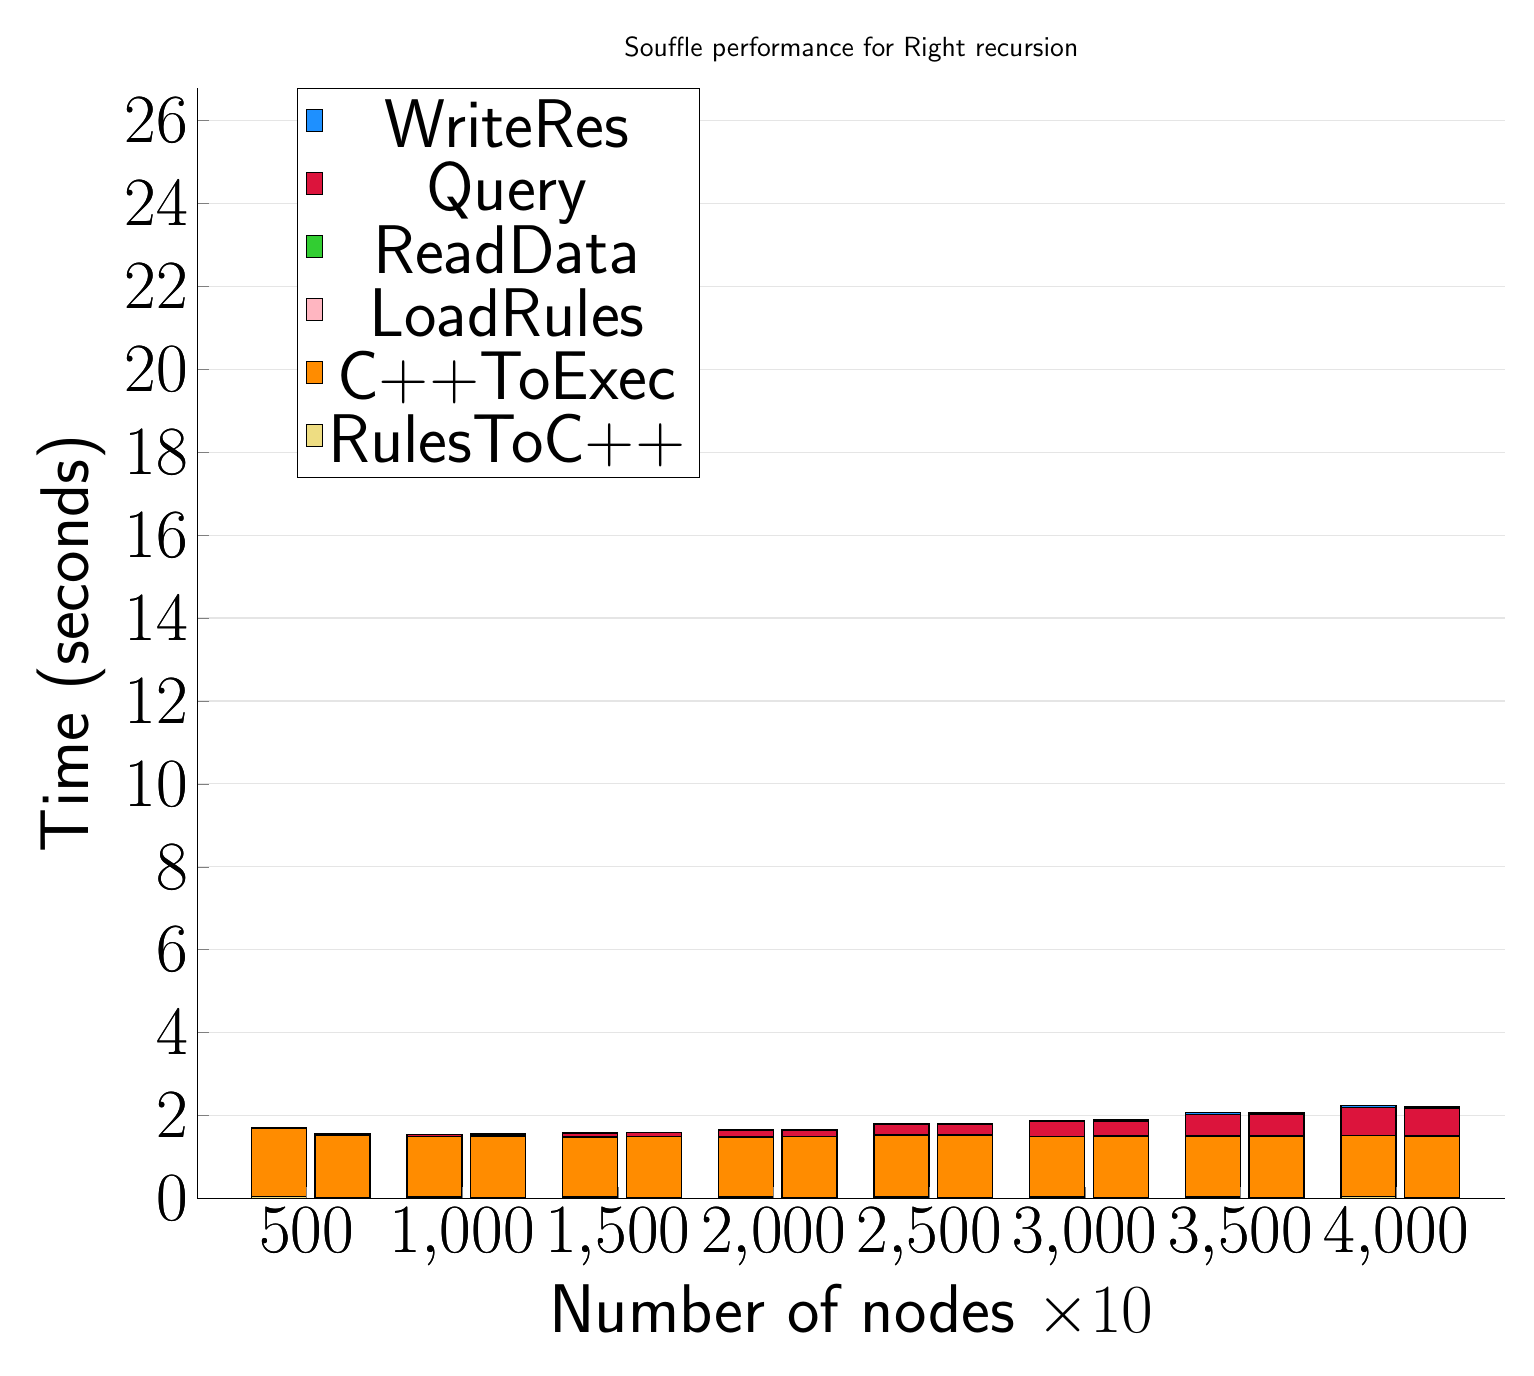
\begin{tikzpicture}
\begin{axis}[
   ybar stacked,
   title={Souffle performance for Right recursion},
   bar shift=-10pt,
   width=1.5\textwidth,
   bar width=0.7cm,
   ymajorgrids, tick align=inside,
   major grid style={draw=gray!20},
   xtick=data,
   ymin=0, ymax=26.78465,
   axis x line*=bottom,
   axis y line*=left,
   enlarge x limits=0.1,
   legend style={
       at={(0.23, 1)},
       anchor=north,
       legend columns=1,
       font=\Huge,
   },
   ylabel={Time (seconds)},
   xlabel={Number of nodes $\times 10$},
   label style={font=\Huge},
   tick label style={font=\Huge},
]
\addlegendimage{fill=DodgerBlue, draw=black, line width=0.2pt}
\addlegendentry{WriteRes}
\addlegendimage{fill=Crimson, draw=black, line width=0.2pt}
\addlegendentry{Query}
\addlegendimage{fill=LimeGreen, draw=black, line width=0.2pt}
\addlegendentry{ReadData}
\addlegendimage{fill=LightPink, draw=black, line width=0.2pt}
\addlegendentry{LoadRules}
\addlegendimage{fill=DarkOrange, draw=black, line width=0.2pt}
\addlegendentry{C++ToExec}
\addlegendimage{fill=LightGoldenrod, draw=black, line width=0.2pt}
\addlegendentry{RulesToC++}
\addplot +[fill=LightGoldenrod, draw=black, line width=0.5pt] coordinates {
    (500, 0.04799997806549072)
    (1000, 0.039999961853027344)
    (1500, 0.039999985694885255)
    (2000, 0.04100000858306885)
    (2500, 0.041999983787536624)
    (3000, 0.040999984741210936)
    (3500, 0.041999983787536624)
    (4000, 0.045999979972839354)
};
\addplot +[fill=DarkOrange, draw=black, line width=0.5pt] coordinates {
    (500, 1.6460000276565552)
    (1000, 1.4549999952316284)
    (1500, 1.4470000267028809)
    (2000, 1.4480000019073487)
    (2500, 1.4880000352859497)
    (3000, 1.450000023841858)
    (3500, 1.4619999885559083)
    (4000, 1.4680000066757202)
};
\addplot +[fill=LightPink, draw=black, line width=0.5pt] coordinates {
    (500, 1.38167e-05)
    (1000, 0.0)
    (1500, 1.0029199999999999e-05)
    (2000, 0.0)
    (2500, 0.0)
    (3000, 0.0)
    (3500, 0.0)
    (4000, 0.0)
};
\addplot +[fill=LimeGreen, draw=black, line width=0.5pt] coordinates {
    (500, 0.0016663899999999998)
    (1000, 0.002681325)
    (1500, 0.004024725)
    (2000, 0.0051271089999999995)
    (2500, 0.005317072000000001)
    (3000, 0.007177399000000001)
    (3500, 0.008933162)
    (4000, 0.009224778999999999)
};
\addplot +[fill=Crimson, draw=black, line width=0.5pt] coordinates {
    (500, 0.013788249999999998)
    (1000, 0.043550229999999995)
    (1500, 0.09119671)
    (2000, 0.15749960000000002)
    (2500, 0.2547122)
    (3000, 0.3608934999999999)
    (3500, 0.5217668)
    (4000, 0.6720126999999999)
};
\addplot +[fill=DodgerBlue, draw=black, line width=0.5pt] coordinates {
    (500, 0.0011587053000000002)
    (1000, 0.0031119749999999995)
    (1500, 0.006536662)
    (2000, 0.011354809999999998)
    (2500, 0.017644890000000003)
    (3000, 0.025152269999999997)
    (3500, 0.03459061)
    (4000, 0.04520355)
};
\end{axis}
\begin{axis}[
   ybar stacked,
   bar shift=13pt,
   width=1.5\textwidth,
   bar width=0.7cm,
   ymajorgrids, tick align=inside,
   major grid style={draw=none},
   xtick=data,
   ymin=0, ymax=26.78465,
   axis x line*=none,
   axis y line*=none,
   enlarge x limits=0.1,
   label style={font=\Huge},
   tick label style={font=\Huge},
]
\addplot +[fill=LightGoldenrod, draw=black, line width=0.5pt] coordinates {
    (500, 0.031000000000000007)
    (1000, 0.030000000000000006)
    (1500, 0.030000000000000006)
    (2000, 0.030000000000000006)
    (2500, 0.030000000000000006)
    (3000, 0.030000000000000006)
    (3500, 0.030000000000000006)
    (4000, 0.031000000000000007)
};
\addplot +[fill=DarkOrange, draw=black, line width=0.5pt] coordinates {
    (500, 1.5050000000000001)
    (1000, 1.475)
    (1500, 1.4629999999999996)
    (2000, 1.465)
    (2500, 1.5029999999999997)
    (3000, 1.47)
    (3500, 1.472)
    (4000, 1.4719999999999998)
};
\addplot +[fill=LightPink, draw=black, line width=0.5pt] coordinates {
    (500, 1.36e-05)
    (1000, 0.0)
    (1500, 0.0)
    (2000, 0.0)
    (2500, 0.0)
    (3000, 0.0)
    (3500, 0.0)
    (4000, 0.0)
};
\addplot +[fill=LimeGreen, draw=black, line width=0.5pt] coordinates {
    (500, 0.0016648)
    (1000, 0.0026628999999999997)
    (1500, 0.0039992)
    (2000, 0.0051063)
    (2500, 0.0052884)
    (3000, 0.007152)
    (3500, 0.008894599999999999)
    (4000, 0.009185300000000002)
};
\addplot +[fill=Crimson, draw=black, line width=0.5pt] coordinates {
    (500, 0.0137789)
    (1000, 0.043477999999999996)
    (1500, 0.0910056)
    (2000, 0.1572095)
    (2500, 0.25384290000000004)
    (3000, 0.3597397)
    (3500, 0.5200339000000002)
    (4000, 0.6699740999999999)
};
\addplot +[fill=DodgerBlue, draw=black, line width=0.5pt] coordinates {
    (500, 0.0011494)
    (1000, 0.0030997999999999998)
    (1500, 0.0064777)
    (2000, 0.011168899999999999)
    (2500, 0.017463600000000003)
    (3000, 0.024829499999999997)
    (3500, 0.033634)
    (4000, 0.044295900000000006)
};
\end{axis}
\end{tikzpicture}

\end{document}
